% Provenance (never printed): see sources/outline_sources.md (Year 3: the
% Rayleigh number; thermal boundary layers; slab pull and ridge push; plumes;
% post-glacial rebound and mantle viscosity). Brief: sources/book5/BRIEFS.md,
% ch. 6. Curves from figdata/bachelor-3/convection_scaling.py (PREM read only),
% gia_relaxation.py and ridge_push.py (on plate_cooling.py). Exercise and
% problem values in the Book 5 scratch calculator calc/ch06.py.
\chapter{प्रावार संवहन और प्लेट-चालक बल}\label{ch:b3:mantle-convection}

उत्तरी स्वीडन का तट लगभग एक सेंटीमीटर प्रति
वर्ष की दर से समुद्र से ऊपर उठ रहा है, उस हिमचादर के पिघल जाने के दस हज़ार वर्ष बाद, जिसने उसे ढक रखा था;
हडसन खाड़ी के तट भी उतनी ही तेज़ी से ऊपर उठते हैं। उन्हें धकेलने वाला कोई और नहीं, केवल प्रावार है,
जो धीरे-धीरे उस स्थान के नीचे वापस बहता है जिसे हिमचादर ने दबाया था। ज़मीन जिस दर से
वापस उछलती है, वह प्रावार की श्यानता का माप देती है, और वही
श्यानता तय करती है कि प्रावार कितनी तेज़ी से संवहन करता है और प्लेटें कितनी तेज़ी से चलती हैं। यह अध्याय पूछता है
कि ठोस प्रावार आख़िर संवहन क्यों करता है, और पृथ्वी की ऊष्मा ढोने के लिए उसे कितनी तेज़ी से बहना होगा,
कौन-से बल प्लेटों को चलाते हैं, और ज़मीन का प्रतिक्षेप
प्रावार की श्यानता के बारे में क्या बताता है।
% ledger: vestol19:umea, zhao12:fenno, sella07:gia

\begin{recall}
श्यानता, श्यान तरल का विसर्पी प्रवाह (स्टोक्स समीकरण
$\nabla p = \eta\nabla^2\mathbf u$, $\nabla\cdot\mathbf u = 0$), गोले के लिए स्टोक्स का नियम,
रेनॉल्ड्स संख्या और उत्प्लावकता भौतिकी की पुस्तकों के स्नातक खंडों में हैं। प्रावार संवहन और समस्थितिक प्रतिक्षेप का
परिचय उच्च विद्यालय की पुस्तक (कक्षा 12) में हो चुका है, और
कटक-धक्का तथा स्लैब-खिंचाव उसके कक्षा 11 वाले भाग में।
ऊष्मीय सीमा-परत, ऊष्मीय स्थलमंडल और प्रावार रुद्धोष्म
पुस्तक 3 (स्नातक वर्ष 1) में हैं, उसके पृथ्वी के ऊष्मा-बजट वाले अध्याय में; हॉटस्पॉट,
प्रावार-स्तंभ और बृहत आग्नेय प्रांत उसके हॉटस्पॉट वाले अध्याय में।
\omterm{def:b3:lithosphere-thermal-models:half-space}{अर्ध-समष्टि शीतलन मॉडल} \cref{ch:b3:lithosphere-thermal-models} में है,
\omterm{def:b3:gravity-geodesy:flexure}{स्थलमंडलीय आनमन} \cref{ch:b3:gravity-geodesy} में है,
और \omterm{def:b3:seismology-imaging:tomography}{भूकंपीय टोमोग्राफ़ी} \cref{ch:b3:seismology-imaging} में।
\end{recall}

\section{प्रावार संवहन क्यों करता है}

प्रावार ठोस है: वह S तरंगों को संचरित करता है। फिर भी लाखों वर्षों में वह
अत्यधिक श्यानता वाले तरल की तरह विसर्पित होता है, और नीचे से गरम तथा ऊपर से ठंडी
तरल-परत स्थिर रह सकती है, जिसमें ऊष्मा चालन से आर-पार जाती है,
या वह पलट सकती है। आकार $d$ का गरम तरल-पिंड, जो अपने परिवेश से
$\rho\alpha\,\Delta T$ से हल्का है और ऊपर उठता है, जिसकी चाल कोटि
$\rho g\alpha\,\Delta T d^2/\eta$ की होती है; यह अपनी ऊष्मा विसरण से खोता है, जिसमें लगने वाला समय
कोटि $d^2/\kappa$ का होता है। यदि यह ठंडा होने से पहले परत के आर-पार ऊपर उठ सके,
तो परत पलट जाती है।

\begin{definition}[रैले संख्या]\label{def:b3:mantle-convection:rayleigh}
किसी तरल-परत के लिए, जिसकी मोटाई $d$, घनत्व $\rho$, ऊष्मीय प्रसार
गुणांक $\alpha$, तापीय विसरणता $\kappa$ और श्यानता $\eta$ है, गुरुत्व $g$ के अधीन,
$\Delta T$ तापमान-अंतर के साथ, उसके आधार और
ऊपरी सतह के बीच, \emph{रैले संख्या}\index{रैले संख्या} होती है
\[
  \mathrm{Ra} = \frac{\rho g\alpha\,\Delta T d^3}{\kappa\eta},
\]
यह विसरण काल $d^2/\kappa$ का
उत्प्लावी उत्थान काल $\eta/(\rho g\alpha\,\Delta Td)$ से अनुपात है।
\end{definition}

\begin{definition}[क्रांतिक रैले संख्या]\label{def:b3:mantle-convection:critical}
\emph{क्रांतिक रैले संख्या}\index{क्रांतिक रैले संख्या}
$\mathrm{Ra}_c$ किसी परत के लिए \omterm{def:b3:mantle-convection:rayleigh}{रैले संख्या} का वह मान है, जिसके ऊपर
विराम-अवस्था का एक छोटा विक्षोभ संवहन में बढ़ जाता है, और जिसके नीचे
वह क्षीण होकर लुप्त हो जाता है।
\end{definition}

\begin{proposition}[संवहन का आरंभ]\label{prop:b3:mantle-convection:onset}
किसी ऐसी परत के लिए, जिसकी ऊपरी और निचली सतहें अपरूपण प्रतिबल से मुक्त हैं और
स्थिर तापमानों पर रखी गई हों, क्षैतिज तरंग-संख्या $k$ (इकाई $1/d$ में) का विक्षोभ
बढ़ता है जब $\mathrm{Ra} > (\pi^2 + k^2)^3/k^2$ हो। दाहिने पक्ष का न्यूनतम
$k = \pi/\sqrt2$ पर मिलता है, जो यह देता है:
\[
  \mathrm{Ra}_c = \frac{27\pi^4}{4} \approx 657.5,
\]
और पहले उभरने वाले संवहन-कोष्ठ $2\sqrt2\,d$ चौड़े होते हैं। दृढ़ सीमाओं के बीच
$\mathrm{Ra}_c \approx 1708$।
\end{proposition}

\admitted
इसके पीछे का रैखिक स्थायित्व विश्लेषण, ऊष्मा और स्टोक्स
समीकरणों का चालन-अवस्था के सापेक्ष विक्षोभ, भौतिकी की पुस्तकों में
संवहन के विवेचन में है; अभ्यास 11 न्यूनतम की जाँच करता है।

नीचे का चित्र संवहनी परत दिखाता है। प्रावार के मान, कोर–प्रावार सीमा की गहराई
$d = \qty{2891}{km}$, प्रावार का माध्य घनत्व
\qty{4476}{kg.m^{-3}}, और $g$ का मान 9.8 और
\qty{10.7}{m.s^{-2}} के बीच, ये सब भूकंपीय पृथ्वी मॉडल PREM से लिए गए हैं; $\alpha =
\qty{3.1e-5}{K^{-1}}$ और $\Delta T = \qty{1450}{K}$ का मान
\cref{ch:b3:lithosphere-thermal-models} के प्लेट मॉडल से; $\kappa = \qty{e-6}{m^2.s^{-1}}$;
और $\eta$ का मान \num{e21} और \qty{e22}{Pa.s} के बीच है (\cref{sec:b3:mantle-convection:gia} देखिए),
इससे $\mathrm{Ra}$ का मान \num{4.9e6} और \num{4.9e7} के बीच आता है, जो क्रांतिक मान का
लगभग सात हज़ार से सत्तर हज़ार गुना है। प्रावार संवहन किए बिना नहीं रह सकता।
% ledger: data:prem, honda04:gdh1, delaney86:properties, mitrovica96:haskell, milne04:bifrost

\begin{omfigure}
\begin{tikzpicture}[font=\scriptsize, x=1cm, y=1cm]
\fill[blue!10] (0,3.4) rectangle (10,3.0);
\fill[red!12] (0,0) rectangle (10,0.4);
\draw[thick] (0,0) rectangle (10,3.4);
\node[above] at (5,3.4) {ठंडा ऊपरी सिरा, $T_0$};
\node[below] at (5,0) {गरम आधार, $T_0 + \Delta T$};
\foreach \c/\s in {1.25/1, 3.75/-1, 6.25/1, 8.75/-1} {
  \draw[gray!70!black, thick] (\c,1.7) ellipse[x radius=0.95, y radius=1.05];
  \draw[->, gray!70!black, thick] ({\c+0.25*\s},2.75) -- ({\c-0.3*\s},2.75);
  \draw[->, gray!70!black, thick] ({\c-0.25*\s},0.65) -- ({\c+0.3*\s},0.65);
}
\draw[->, red!70!black, very thick] (2.5,0.45) -- (2.5,2.9);
\draw[->, red!70!black, very thick] (7.5,0.45) -- (7.5,2.9);
\draw[->, blue!70!black, very thick] (5,2.95) -- (5,0.5);
\node[red!70!black, fill=white, inner sep=1pt, align=center] at (2.5,1.7) {गरम\\उत्स्रवण};
\node[red!70!black, fill=white, inner sep=1pt, align=center] at (7.5,1.7) {गरम\\उत्स्रवण};
\node[blue!70!black, fill=white, inner sep=1pt, align=center] at (5,1.7) {ठंडा\\अधःस्रवण};
\draw[<->] (10.3,0) -- (10.3,3.4) node[midway, right] {$d$};
\draw[<->] (-0.25,3.0) -- (-0.25,3.4) node[midway, left] {$\delta$};
\draw[<->] (-0.25,0) -- (-0.25,0.4) node[midway, left] {$\delta$};
\node[anchor=west] at (10.6,3.2) {ऊपरी सीमा-परत};
\node[anchor=west] at (10.6,0.2) {निचली सीमा-परत};
\end{tikzpicture}

\par\smallskip{\small नीचे से गरम और ऊपर से ठंडी की गई परत में संवहन।
ऊष्मा मोटाई $\delta$ वाली पतली सीमा-परतों को चालन द्वारा पार करती है;
बीच में अच्छी तरह मिश्रित आंतरिक भाग उसे प्रवाह द्वारा ले जाता है। ठंडी चादरें
ऊपरी परत से अलग होकर डूबती हैं; गरम चादरें
निचली परत से ऊपर उठती हैं।}\label{fig:b3:mantle-convection:cell}
\end{omfigure}

प्रावार भीतर से भी गरम होता है, रेडियोधर्मी तत्वों के क्षय से,
और नीचे से, क्रोड द्वारा। केवल भीतर से गरम की गई परत में
आधार पर कोई गरम सीमा-परत नहीं होती: उसका प्रवाह ऊपर से डूबती ठंडी चादरों द्वारा
चालित होता है, और ऊपर उठता प्रवाह एक चौड़ी, निष्क्रिय वापसी है। स्लैब ऐसी ही चादरें हैं, और
प्लूम को क्रोड से आने वाली ऊष्मा चाहिए।

\section{सीमा-परतें और संवहन की प्रबलता}

\begin{definition}[नुसेल्ट संख्या]\label{def:b3:mantle-convection:nusselt}
किसी संवहनी परत की \emph{नुसेल्ट संख्या}\index{नुसेल्ट संख्या} उस परत से होकर गुजरने वाले
ऊष्मा-प्रवाह को, उसी परत से केवल चालन द्वारा वहन होने वाले ऊष्मा-प्रवाह से भाग देने पर
मिलने वाला अनुपात है, $\mathrm{Nu} = q\,d/(k\,\Delta T)$।
\end{definition}

\begin{theorem}[संवहन का सीमा-परत स्केलन]\label{thm:b3:mantle-convection:scaling}
$\mathrm{Ra} \gg \mathrm{Ra}_c$ पर संवहन करती किसी परत में, यदि हर ऊष्मीय
सीमा-परत तब तक बढ़ती है जब तक उसकी अपनी \omterm{def:b3:mantle-convection:rayleigh}{रैले संख्या}, जो उसकी मोटाई
$\delta$ और उस पर तापमान-गिरावट $\Delta T/2$ पर आधारित है, वह
$\mathrm{Ra}_c$ तक पहुँच जाती है, तब
\[
  \delta = d\Bigl(\frac{2\mathrm{Ra}_c}{\mathrm{Ra}}\Bigr)^{1/3},\qquad
  \mathrm{Nu} = \frac12\Bigl(\frac{\mathrm{Ra}}{2\mathrm{Ra}_c}\Bigr)^{1/3},
  \qquad
  u = \frac\kappa d\Bigl(\frac{\mathrm{Ra}}{2\mathrm{Ra}_c}\Bigr)^{2/3},
\]
जहाँ $u$ प्रवाह का वेग-स्केल है, जिसे इस शर्त से परिभाषित किया गया है कि
परत $\delta$ तक बढ़ती है, जबकि द्रव कोष्ठ को पार करता है। यही
\emph{संवहन का सीमा-परत स्केलन}\index{संवहन का सीमा-परत स्केलन} कहलाता है।
\end{theorem}

\begin{proof}
अंदरूनी भाग अच्छी तरह मिश्रित है और माध्य तापमान पर है, इसलिए हर सीमा-परत
$\Delta T$ का आधा वहन करती है। इसकी \omterm{def:b3:mantle-convection:rayleigh}{रैले संख्या} है $\rho g\alpha(\Delta T/2)
\delta^3/(\kappa\eta) = \mathrm{Ra}\,(\delta/d)^3/2$; इसे
$\mathrm{Ra}_c$ के बराबर रखने पर $\delta$ प्राप्त होता है। ऊष्मा-प्रवाह परत के आर-पार चालन द्वारा होता है,
$q = k(\Delta T/2)/\delta$ है, अतः $\mathrm{Nu} = qd/(k\Delta T) = d/(2\delta)$।
सीमा-परत विसरण द्वारा मोटाई $\delta$ तक बढ़ती है, इसके लिए लगा समय
$\delta^2/\kappa$ है; ऊपर का द्रव, जिसकी चौड़ाई कोटि $d$ है, कोष्ठ को
$d/u$ समय में पार करता है। दोनों समयों को बराबर रखने पर, $u = \kappa d/\delta^2 =
(\kappa/d)(d/\delta)^2$।
\end{proof}

ऊष्मा-प्रवाह केवल $\mathrm{Ra}$ के घनमूल के रूप में बढ़ता है: श्यानता
सौ गुना कम हो, तो ऊष्मा पाँच गुने से भी कम अधिक मिलती है।
प्रावार की $\mathrm{Ra} = \num{4.9e7}$ के साथ स्केलन देता है $\delta \approx \qty{87}{km}$,
$\mathrm{Nu} \approx 17$, ऊष्मा-प्रवाह $\mathrm{Nu}\,k\Delta T/d \approx
\qty{26}{mW.m^{-2}}$, जहाँ $k = \qty{3.1}{W.m^{-1}.K^{-1}}$ है, और $u \approx
\qty{1.2}{cm/yr}$ (नीचे का चित्र देखिए)। सीमा-परत उतनी ही मोटी है, जितनी
\cref{ch:b3:lithosphere-thermal-models} में बताई सागरीय प्लेट, \qty{95}{km};
आज की प्लेटों की वर्ग-माध्य-मूल चालें \qty{1.1}{cm/yr} (दक्षिण
अमेरिका) से लेकर \qty{7.5}{cm/yr} (कोकोस) तक हैं, और संपूर्ण
स्थलमंडल के लिए \qty{4.4}{cm/yr}। पृथ्वी का माध्य ऊष्मा-प्रवाह, \qty{92}{mW.m^{-2}}, स्केलन के
तीन से चार गुना है: प्रावार के भीतर उत्पन्न ऊष्मा, जिसे नीचे से गरम परत छोड़ देती है,
और कोटि-एक के वे स्थिरांक, जिन्हें स्केलन नज़रअंदाज़ करता है, दोनों ही योगदान देते हैं।
एकल निवेश वाले नियम के लिए परिमाण-कोटियाँ सही हैं:
प्लेटें उस प्रावार की ऊपरी सीमा-परत हैं जिसकी $\mathrm{Ra}
\sim 10^7$ है।
% ledger: nnr56:rms, b2dd10:continents, honda04:gdh1

\begin{omfigure}
\begin{tikzpicture}
\begin{groupplot}[group style={group size=1 by 2, vertical sep=2.5cm},
  omrecord, width=0.86\linewidth, height=0.40\linewidth, xmode=log, ymode=log,
  xmin=100, xmax=1e10, xlabel={रैले संख्या $\mathrm{Ra}$}]
\nextgroupplot[ylabel={नुसेल्ट संख्या}, ymin=0.3, ymax=300,
  title={(क) चालन-प्रवाह की इकाई में ऊष्मा-प्रवाह}, title style={font=\small}]
% computed in figdata/bachelor-3/convection_scaling.py; ledger: data:prem, honda04:gdh1
\addplot[omDef, thick] table[x=ra, y=nu] {figdata/out/bachelor-3-convection_scaling-conduction.dat};
\addplot[red!70!black, thick] table[x=ra, y=nu] {figdata/out/bachelor-3-convection_scaling-scaling.dat};
\addplot[gray, densely dashed, unbounded coords=jump] table[x=ra, y=y] {figdata/out/bachelor-3-convection_scaling-band.dat};
\draw[gray, densely dotted] (axis cs:657.5,0.3) -- (axis cs:657.5,1);
\node[font=\scriptsize, anchor=west] at (axis cs:700,0.45) {$\mathrm{Ra}_c$};
\node[font=\scriptsize, anchor=south west, omDef] at (axis cs:115,1.08) {चालन};
\node[font=\scriptsize, anchor=north west, red!70!black] at (axis cs:3e4,0.95) {$\tfrac12(\mathrm{Ra}/2\mathrm{Ra}_c)^{1/3}$};
\node[font=\scriptsize, fill=white, inner sep=1pt] at (axis cs:1.55e7,120) {प्रावार};
\nextgroupplot[ylabel={वेग (\unit{cm/yr})}, ymin=1e-3, ymax=100,
  title={(ख) $d = \qty{2891}{km}$ के लिए वेग-स्केल}, title style={font=\small}]
\addplot[red!70!black, thick] table[x=ra, y=u] {figdata/out/bachelor-3-convection_scaling-scaling.dat};
\addplot[gray, densely dashed, unbounded coords=jump] table[x=ra, y=y] {figdata/out/bachelor-3-convection_scaling-band.dat};
\addplot[blue!70, thick, dash dot, unbounded coords=jump] table[x=ra, y=u] {figdata/out/bachelor-3-convection_scaling-plates.dat};
\node[font=\scriptsize, anchor=south west, blue!60!black] at (axis cs:150,7.6) {सबसे तेज़ प्लेट};
\node[font=\scriptsize, anchor=north west, blue!60!black] at (axis cs:150,1.0) {सबसे धीमी प्लेट};
\node[font=\scriptsize, fill=white, inner sep=1pt] at (axis cs:1.55e7,0.004) {प्रावार};
\end{groupplot}
\end{tikzpicture}

\par\smallskip{\small संवहन स्केलन। (क) $\mathrm{Ra}_c$ से नीचे परत चालन करती है
($\mathrm{Nu} = 1$); उससे कहीं ऊपर सीमा-परत नियम, जो
$\mathrm{Ra} = 16\,\mathrm{Ra}_c \approx \num{1.1e4}$ से खींचा गया है, जहाँ यह $\mathrm{Nu} = 1$ देता है (इनके बीच
संवहन धीरे-धीरे आरंभ होता है)। (ख) वेग-स्केल प्रावार की गहराई
और $\kappa = \qty{e-6}{m^2.s^{-1}}$ के लिए, साथ में आज की प्लेट-गतियों की
परास (बिंदु-डैश रेखा) दिखाई गई है। कटी रेखाएँ प्रावार की \omterm{def:b3:mantle-convection:rayleigh}{रैले संख्या} की
सीमा बताती हैं, श्यानताओं \num{e22} और \qty{e21}{Pa.s} के लिए।}\label{fig:b3:mantle-convection:scaling}
\end{omfigure}

\section{प्लेट पर बल}

प्लेट स्थिर चाल से चलती है: उस पर लगने वाले बल संतुलित होते हैं। तीन बल
उसे उसके किनारों और आधार से चलाते हैं या उसका विरोध करते हैं (नीचे का चित्र देखिए)। वह बल जो
डूबता स्लैब अपनी प्लेट पर लगाता है, वह स्लैब-खिंचाव कहलाता है, और यह आता है
गरम प्रावार में ठंडे स्लैब के अतिरिक्त घनत्व से। कटक-धक्का, ऊँचे और गरम कटक का
बगल की ठंडी प्लेट पर लगने वाला उसका धक्का है, जो
\cref{ch:b3:lithosphere-thermal-models} में दिए \omterm{def:b3:lithosphere-thermal-models:half-space}{अर्ध-समष्टि शीतलन मॉडल} से निकलता है।

\begin{omfigure}
\begin{tikzpicture}[font=\scriptsize, x=1cm, y=1cm]
\fill[orange!12] (0,-0.6) rectangle (12.6,-6.0);
\fill[blue!8] (0,0) -- (0,-0.6) .. controls (3,-1.0) and (6,-1.25) .. (8.4,-1.3) -- (8.9,-1.9) -- (10.6,-0.2) -- (10.6,0) -- cycle;
\fill[gray!35] (0,-0.6) .. controls (3,-1.0) and (6,-1.25) .. (8.4,-1.3) -- (8.9,-1.9) -- (11.2,-5.0) -- (10.3,-5.6) -- (8.4,-2.9) .. controls (6,-2.85) and (3,-2.4) .. (0.2,-0.95) -- cycle;
\fill[gray!18] (10.6,-0.2) -- (12.6,0.1) -- (12.6,-2.5) -- (11.7,-2.5) -- (8.9,-1.9) -- cycle;
\draw[thick] (0,-0.6) .. controls (3,-1.0) and (6,-1.25) .. (8.4,-1.3) -- (8.9,-1.9) -- (11.2,-5.0);
\draw (0.2,-0.95) .. controls (3,-2.4) and (6,-2.85) .. (8.4,-2.9) -- (10.3,-5.6);
\draw[blue!50!black] (0,0) -- (12.6,0);
\node at (0.4,0.2) {कटक};
\node at (4.5,-1.8) {महासागरीय प्लेट};
\node at (11.9,-0.9) {ऊपरी प्लेट};
\node[rotate=-53] at (10.1,-4.0) {स्लैब};
\node at (3,-4.6) {प्रावार};
\draw[->, very thick, red!70!black] (0.6,-0.93) -- (2.2,-0.93);
\node[red!70!black] at (1.5,-0.35) {कटक-धक्का};
\draw[->, very thick, red!70!black] (10.9,-5.6) -- (11.5,-6.4) node[right] {स्लैब-खिंचाव};
\draw[->, very thick, blue!60!black] (6.0,-3.25) -- (4.8,-3.25) node[below, pos=0.5] {आधारी कर्षण};
\draw[->, very thick, blue!60!black] (8.9,-4.3) -- (8.45,-3.65) node[left] {स्लैब-प्रतिरोध};
\draw[->, thick] (4.2,0.45) -- (6.6,0.45) node[right] {प्लेट-गति};
\end{tikzpicture}

\par\smallskip{\small महासागरीय प्लेट पर बल: कटक-धक्का और स्लैब-खिंचाव
उसे चलाते हैं (लाल); \omterm{def:b3:mantle-convection:basal-drag}{आधारी कर्षण}, जहाँ प्लेट अपने नीचे के प्रावार से तेज़ चलती है,
और डूबते स्लैब के प्रति प्रावार का श्यान प्रतिरोध उसका विरोध करते हैं
(नीला)।}\label{fig:b3:mantle-convection:forces}
\end{omfigure}

\begin{proposition}[कटक-धक्का बल]\label{prop:b3:mantle-convection:ridge-push}
\omterm{def:b3:lithosphere-thermal-models:half-space}{अर्ध-समष्टि शीतलन मॉडल} में, प्रावार का तापमान $T_m$, पृष्ठ का
तापमान $T_0$ और समस्थितिक क्षतिपूर्ति हों, तो आयु $t$ की प्लेट पर कटक के स्तंभ
द्वारा कटक की प्रति इकाई लंबाई पर लगने वाला क्षैतिज बल,
\emph{कटक-धक्का बल}\index{कटक-धक्का बल}, इस प्रकार है:
\[
  F_{rp} = g\rho_m\alpha(T_m - T_0)\kappa t\Bigl[1 + \frac{2\rho_m\alpha(T_m
  - T_0)}{\pi(\rho_m - \rho_w)}\Bigr].
\]
\end{proposition}

\begin{proof}
मान लीजिए $y$ कटक पर समुद्र-तल के नीचे की गहराई है, और $w$ आयु $t$ वाले तल का अवधसान,
$\theta(z) = T_m - T(z)$ प्लेट में गहराई $z = y - w$ पर तापमान-न्यूनता है,
और $\Theta(z) = \int_0^z\theta$।
कटक का स्तंभ घनत्व $\rho_m$ वाला प्रावार $y = 0$ से रखता है; पुराना स्तंभ
$w$ तक जल रखता है, फिर घनत्व $\rho_m(1 + \alpha\theta)$ वाली प्लेट।
शैलस्थैतिक दाबों का अंतर $P_r - P_t = (\rho_m - \rho_w)gy$ है, जब $y < w$ हो,
और उससे नीचे,
\[
  P_r - P_t = (\rho_m - \rho_w)gw - \rho_mg\alpha\,\Theta(z)
  = \rho_mg\alpha\bigl(\Theta(\infty) - \Theta(z)\bigr),
\]
समस्थिति से, $(\rho_m - \rho_w)w = \rho_m\alpha\Theta(\infty)$ है। बल गहराई पर दाब-अंतर का
समाकल है; दूसरे भाग का खंडशः समाकलन करने पर
निम्नलिखित प्राप्त होता है,
\[
  F_{rp} = \tfrac12(\rho_m - \rho_w)gw^2 + \rho_mg\alpha\int_0^\infty
  z\,\theta(z)\,\mathrm dz .
\]
अर्ध-समष्टि के लिए, $\theta = (T_m - T_0)\operatorname{erfc}(z/2\sqrt{\kappa
t})$ और $\int_0^\infty x\operatorname{erfc}x\,\mathrm dx = 1/4$, अतः
समाकल $(T_m - T_0)\kappa t$ है; और $w = 2\rho_m\alpha(T_m -
T_0)\sqrt{\kappa t/\pi}/(\rho_m - \rho_w)$। दोनों पदों को जोड़ने पर
सूत्र प्राप्त होता है।
\end{proof}

कटक-धक्का आयु के साथ रैखिक रूप से बढ़ता है; यह अक्ष पर का कोई धक्का नहीं, बल्कि एक
पूरी ठंडी होती प्लेट पर फैली दाब-प्रवणता है।
\cref{ch:b3:lithosphere-thermal-models} के मानों से, कोष्ठक का मान 1.04 है और $F_{rp} =
\qty{3.8e12}{N.m^{-1}}$ है, \qty{100}{Myr} पर। प्लेट मॉडल में यह
गहराई के साथ बढ़ना रुक जाता है, लगभग \qty{2.3e12}{N.m^{-1}} पर (नीचे का चित्र देखिए)। स्लैब-खिंचाव
इससे बड़ा है: \qty{95}{km} मोटा एक स्लैब, जो औसतन प्रावार से $(T_m - T_0)/2$ ठंडा है,
इसलिए $\rho_m\alpha(T_m - T_0)/2 \approx
\qty{74}{kg.m^{-3}}$ अधिक घना है, \qty{670}{km} तक नीचे लटकता हुआ स्लैब
विस्थापित प्रावार से \qty{4.6e13}{N.m^{-1}} अधिक भार रखता है।
यह कटक-धक्के का बारह गुना है। उस भार का बड़ा भाग उस श्यान प्रावार पर खर्च होता है
जो स्लैब के डूबने का विरोध करता है, और केवल एक भाग ही प्लेट तक पहुँचता है।
% ledger: honda04:gdh1, data:prem

\begin{omfigure}
\begin{tikzpicture}
\begin{axis}[omrecord, width=0.8\linewidth, height=0.42\linewidth,
  xmin=0, xmax=160, ymin=0, ymax=6.5, xlabel={समुद्र-तल की आयु (Myr)},
  ylabel={$F_{rp}$ (\qty{e12}{N.m^{-1}})},
  legend cell align=left,
  legend style={font=\scriptsize, at={(0.03,0.97)}, anchor=north west}]
% computed in figdata/bachelor-3/ridge_push.py; ledger: honda04:gdh1
\addplot[omDef, thick] table[x=t, y=hs] {figdata/out/bachelor-3-ridge_push-force.dat};
\addlegendentry{अर्ध-समष्टि}
\addplot[red!70!black, thick, densely dashed] table[x=t, y=pl] {figdata/out/bachelor-3-ridge_push-force.dat};
\addlegendentry{प्लेट, $L = \qty{95}{km}$}
\end{axis}
\end{tikzpicture}

\par\smallskip{\small प्लेट की आयु के विरुद्ध \omterm{prop:b3:mantle-convection:ridge-push}{कटक-धक्का बल}, जिसे
\cref{ch:b3:lithosphere-thermal-models} के दो शीतलन मॉडलों से, संख्यात्मक
दाब-अंतर के समाकलन द्वारा परिकलित (अर्ध-समष्टि वक्र
प्रतिज्ञप्ति का बंद रूप है)।}\label{fig:b3:mantle-convection:ridge-push}
\end{omfigure}

\begin{definition}[आधारी कर्षण]\label{def:b3:mantle-convection:basal-drag}
\emph{आधारी कर्षण}\index{आधारी कर्षण} वह प्रति इकाई क्षेत्रफल का अपरूपण बल है जो
किसी प्लेट के नीचे का प्रावार उसके आधार पर लगाता है। $u$ चाल से चलती प्लेट के लिए
मोटाई $h$ और श्यानता $\eta$ की परत पर, जिसका आधार स्थिर है,
यह $\eta u/h$ है, गति के विपरीत; यह प्लेट को वहाँ चलाता है जहाँ
उसके नीचे का प्रावार प्लेट से तेज़ चलता है।
\end{definition}

कौन-से बल मायने रखते हैं, यह स्वयं प्लेटों से पढ़ा जा सकता है। बलाघूर्ण-संतुलन
प्रत्येक प्लेट पर, प्लेट-गतियों से मिलाया गया, कहता है कि डूबते स्लैब पर कार्य करने वाले बल
महासागरीय प्लेटों की चाल नियंत्रित करते हैं, और अन्य किसी भी बल से लगभग दस गुना
प्रबल हैं; और यह कि आधार पर का प्रतिरोध महाद्वीपों के नीचे
महासागरों के नीचे से अधिक है। गतियाँ मेल खाती हैं: सबसे तेज़ प्लेटें, कोकोस
\qty{75}{mm/yr}, नाज़का 70 और प्रशांत \qty{66}{mm/yr} पर, जो महासागरीय
प्लेटें हैं जिनके किनारे लंबी खाइयों में डूबते हैं; सबसे धीमी वे हैं जो बड़े महाद्वीप ढोती हैं:
यूरेशिया 23, उत्तरी अमेरिका 20, दक्षिणी अमेरिका \qty{11}{mm/yr} पर।
% ledger: fu75:slab-pull, nnr56:rms

\section{प्लूम}

प्रावार के आधार से उठती गर्म पट्टें स्तंभों में एकत्र हो जाती हैं: ये
पुस्तक 3 (स्नातक वर्ष 1) वाले प्रावार-स्तंभ हैं, जिनका शीर्ष बड़ा और पूँछ पतली होती है (नीचे का चित्र देखिए)।
हॉटस्पॉट का उभार, जो ज्वालामुखियों के चारों ओर और उनके बहाव की दिशा में समुद्र-तल का चौड़ा उठाव है,
यह मापता है कि उसका प्लूम कितनी उत्प्लावकता लाता है।

\begin{definition}[प्लूम उत्प्लावन अभिवाह]\label{def:b3:mantle-convection:buoyancy-flux}
\emph{प्लूम उत्प्लावन अभिवाह}\index{प्लूम उत्प्लावन अभिवाह} $B$ वह द्रव्यमान न्यूनता है,
जो आसपास के प्रावार के सापेक्ष कोई प्लूम प्रति इकाई
समय में ऊपर ले जाता है; आयतन अभिवाह $Q_v$ और तापमान आधिक्य $\Delta T$ वाले प्लूम के लिए,
$B = \rho\alpha\,\Delta T\,Q_v$।
\end{definition}

\begin{proposition}[उभार से उत्प्लावन अभिवाह]\label{prop:b3:mantle-convection:swell}
यदि कोई पट्टी, जो प्लूम के ऊपर से चाल $u$ से गुज़रती है, ऐसा उभार लिए हो
जिसका पार-काट क्षेत्रफल $A$ है और जिसे उसके नीचे का प्लूम-पदार्थ समस्थितिक रूप से सहारा दे रहा हो,
तो प्लूम का उत्प्लावन अभिवाह होता है:
\[
  B = (\rho_m - \rho_w)\,A\,u .
\]
\end{proposition}

\begin{proof}
समस्थिति के कारण, पटरी के अनुदिश एकांक लंबाई का उभार का वह टुकड़ा, जो
अनुप्रस्थ-काट के क्षेत्रफल $A$ पर समुद्र-तल को ऊपर उठाता है और पानी की जगह शैल ले लेता है,
नीचे के स्तंभ में द्रव्यमान न्यूनता $(\rho_m - \rho_w)A$ से सहारा पाता है।
पट्टी इस टुकड़े को चाल $u$ से दूर ले जाती है, इसलिए स्थायी अवस्था में प्लूम को
प्रति इकाई समय में नए उभार की लंबाई $u$ के लिए यह न्यूनता पूरी करनी होगी।
\end{proof}

उभार की अनुप्रस्थ-काटों से पता चलता है कि हॉटस्पॉटों के उत्प्लावन अभिवाह बीस गुने के दायरे में फैले हैं:
हवाई, सबसे बड़ा, \qty{8.7}{Mg/s}; आइसलैंड
\qty{1.4}{Mg/s}; 37 हॉटस्पॉट मिलाकर लगभग \qty{50}{Mg/s}। उत्प्लावकता का प्रत्येक किलोग्राम
$c_p/\alpha$ जूल अतिरिक्त ऊष्मा है, इसलिए ऊष्मा-अभिवाह $c_pB/\alpha$ है;
जहाँ $c_p = k/(\rho_m\kappa) = \qty{1170}{J.kg^{-1}.K^{-1}}$ और $\alpha =
\qty{3.1e-5}{K^{-1}}$, 37 हॉटस्पॉट लगभग \qty{1.9}{TW} वहन करते हैं, या
\qty{3.7}{mW.m^{-2}} दर से, पृथ्वी के \qty{5.1e14}{m^2} क्षेत्रफल पर बँटकर, जो
प्रवाहों के साथ प्रकाशित \qty{4}{mW.m^{-2}} के निकट है: यह पृथ्वी द्वारा
खोई जाने वाली \qty{47}{TW} का कुछ प्रतिशत है। प्लूम ऊष्मा-बजट के छोटे साझेदार हैं;
शेष ऊष्मा पट्टें वहन करती हैं।
% ledger: sleep90:flux, b2dd10:half-space, honda04:gdh1

\begin{omfigure}
\begin{tikzpicture}[font=\scriptsize, x=1cm, y=1cm]
\fill[orange!12] (0,0) rectangle (11,-5.6);
\fill[gray!35] (0,0) -- (11,0) -- (11,-0.7) -- (0,-0.7) -- cycle;
\fill[red!25] (3.3,-5.6) -- (3.3,-3.4) .. controls (3.3,-2.6) and (1.6,-2.4) .. (1.6,-1.7)
  .. controls (1.6,-0.8) and (5.4,-0.8) .. (5.4,-1.7) .. controls (5.4,-2.4) and (3.7,-2.6) .. (3.7,-3.4) -- (3.7,-5.6) -- cycle;
\fill[red!25] (8.3,-5.6) -- (8.3,-0.75) -- (8.7,-0.75) -- (8.7,-5.6) -- cycle;
\fill[red!40] (8.0,-0.75) -- (8.3,-1.1) -- (8.7,-1.1) -- (10.4,-0.75) -- cycle;
\draw[thick] (0,-5.6) -- (11,-5.6);
\fill[red!45!orange] (0,-5.6) rectangle (11,-6.0);
\fill[red!12] (0,-5.6) rectangle (3.3,-5.25) (3.7,-5.6) rectangle (8.3,-5.25) (8.7,-5.6) rectangle (11,-5.25);
\node[anchor=west] at (0.1,-5.8) {क्रोड};
\node at (3.5,-1.6) {प्लूम-शीर्ष};
\node[anchor=west] at (3.8,-4.4) {पूँछ};
\node[anchor=west] at (8.8,-3.8) {पूँछ};
\node[anchor=west] at (0.1,-0.35) {स्थलमंडल};
\node at (6.0,-3.0) {प्रावार};
\draw[->] (3.5,-5.2) -- (3.5,-3.0);
\draw[->] (8.5,-5.2) -- (8.5,-1.6);
\draw[->, thick] (5.4,-0.35) -- (6.8,-0.35) node[right] {पट्टी-गति};
\draw[blue!50!black] (0,0) .. controls (2.5,0) and (2.6,0.35) .. (3.5,0.35) .. controls (4.4,0.35) and (4.5,0) .. (7,0) .. controls (8,0) and (8.2,0.22) .. (8.5,0.22) .. controls (9.4,0.22) and (10,0.08) .. (11,0.05);
\node[above, align=center] at (3.5,0.4) {उत्थान, फिर बाढ़ बेसाल्ट\\जब शीर्ष पहुँचता है};
\node[above, align=center] at (9.6,0.25) {उभार और\\हॉटस्पॉट-पथ};
\node[anchor=west] at (4.3,-5.4) {गर्म आधारी सीमा-परत};
\end{tikzpicture}

\par\smallskip{\small एक युवा प्लूम (बाएँ) एक बड़े शीर्ष के रूप में ऊपर उठता है, जिसे एक पतली
पूँछ से पोषण मिलता है; जब शीर्ष स्थलमंडल के नीचे फैलता है, तो पृष्ठ ऊपर उठता है और बाढ़ बेसाल्ट
फूट सकते हैं। एक पुराना प्लूम (दाएँ) गतिशील पट्टी के नीचे की एक पूँछ है, जो
एक उभार और एक हॉटस्पॉट-पथ का पोषण करती है। पैमाने के
अनुरूप नहीं।}\label{fig:b3:mantle-convection:plume}
\end{omfigure}

उत्प्लावी प्रावार का एक गोला है, जो श्यान प्रावार में ऊपर उठता है: प्लूम-शीर्ष एक
भौतिकी का स्टोक्स नियम, $v = 2\Delta\rho\,ga^2/(9\eta)$, इसकी चाल का
परिमाण बताता है, कुछ सौ किलोमीटर आर-पार के शीर्ष के लिए प्रति वर्ष एक मीटर का अंश,
(अभ्यास 8) इसलिए वह प्रावार को लाखों वर्षों में पार करता है।

\section{हिमनदीय समस्थितिक समायोजन और प्रावार श्यानता}\label{sec:b3:mantle-convection:gia}

\begin{definition}[हिमनदीय समस्थितिक समायोजन, प्रावार श्यानता]\label{def:b3:mantle-convection:gia}
\emph{हिमनदीय समस्थितिक समायोजन}\index{हिमनदीय समस्थितिक समायोजन} (GIA)
ठोस पृथ्वी का धीमा विरूपण है, और उसके गुरुत्व क्षेत्र तथा
समुद्र-तल में आया वह परिवर्तन है, जब वह हिमचादर के बढ़ने या पिघलने के बाद
समस्थितिक साम्य की ओर लौटती है। \emph{प्रावार श्यानता}\index{प्रावार श्यानता}
वह प्रभावी श्यानता $\eta$ है, जो प्रावार के धीमे, स्थायी
विसर्पण को उन प्रतिबलों से जोड़ती है जो उसे चलाते हैं, हज़ारों वर्षों और उससे अधिक समय में।
\end{definition}

जब कोई हिमचादर पिघलती है, तो उसके पीछे छूटा गड्ढा समस्थितिक साम्य से बाहर होता है:
उसके नीचे प्रावार का दाब आसपास की तुलना में कम होता है, और
प्रावार भीतर की ओर बहकर फ़र्श को फिर ऊपर उठाता है। आज बोथनिया की खाड़ी का तट
उमेआ के निकट \qty{10.3}{mm/yr} तक की दर से ऊपर उठ रहा है; हडसन खाड़ी लगभग
\qty{10}{mm/yr} की दर से, जहाँ बर्फ़ सबसे मोटी थी, जबकि ग्रेट लेक्स के दक्षिण का भू-भाग
1 से \qty{2}{mm/yr} की दर से धँस रहा है, क्योंकि जिस उभार को बर्फ़ ने ऊपर धकेला था,
उसके चारों ओर वह अवधसित हो रहा है। तटों पर पुरानी तटरेखाएँ अब समुद्र के ऊपर खड़ी हैं, यानी
नीचे क्षेत्र-बॉक्स में दिखाए गए उत्थित पुलिन।
% ledger: vestol19:umea, sella07:gia

\begin{theorem}[श्यान अर्ध-समष्टि का शिथिलन]\label{thm:b3:mantle-convection:relaxation}
अर्ध-समष्टि के पृष्ठ पर एक अवनमन $w(x, t) = w_m(t)\cos(2\pi x/\lambda)$ है,
जो एकसमान श्यानता $\eta$ और घनत्व $\rho$ वाले अर्ध-समष्टि का है और जिस पर कोई भार नहीं है,
$w_m(t) = w_m(0)e^{-t/\tau}$ के अनुसार क्षय होता है, जहाँ
\[
  \tau = \frac{4\pi\eta}{\rho g\lambda} .
\]
\end{theorem}

\begin{proof}
मान लीजिए $z$ नीचे की ओर है, $k = 2\pi/\lambda$, और ऐसा स्टोक्स प्रवाह खोजा जाता है जो
गहराई के साथ क्षय हो, जिसका ऊर्ध्वाधर वेग (नीचे की ओर) $v = (C + Dkz)e^{-kz}\cos kx$ है।
असंपीड्यता से क्षैतिज वेग $u = -(D - C - Dkz)e^{-kz}\sin
kx$ प्राप्त होता है। ये फलन $\nabla^4 = 0$ को संतुष्ट करते हैं, जैसा
द्विविमीय में हर स्टोक्स प्रवाह करता है। मुक्त पृष्ठ पर कोई अपरूपण प्रतिबल नहीं होता: $\partial u/\partial
z + \partial v/\partial x = 2k(D - C)\sin kx = 0$ है, $z = 0$ पर; इसलिए $D = C$, और
\[
  v = C(1 + kz)e^{-kz}\cos kx,\quad u = Ckze^{-kz}\sin kx,\quad
  p = 2\eta Cke^{-kz}\cos kx,
\]
दाब इससे प्राप्त होता है: $\partial p/\partial x = \eta\nabla^2u = -2\eta
Ck^2e^{-kz}\sin kx$ (और $\partial p/\partial z = \eta\nabla^2v$ की जाँच होती है)। पृष्ठ पर
$\partial v/\partial z = 0$ है, अतः वहाँ अभिलंब प्रतिबल $-p$ है। किसी अवनमन $w$
के नीचे, अनुपस्थित शैल का भार दाब को $\rho
gw$ से घटा देता है: $p(0) = -\rho gw$; अतः $2\eta Ck = -\rho gw_m$। पृष्ठ
द्रव के साथ चलता है: $\mathrm dw_m/\mathrm dt = v(0) = C = -\rho gw_m/(2\eta k)$, जिसका
हल $\tau = 2\eta k/(\rho g) = 4\pi\eta/(\rho g\lambda)$ के साथ क्षय होता है।
\end{proof}

\begin{definition}[समस्थितिक शिथिलन काल]\label{def:b3:mantle-convection:relaxation-time}
\emph{समस्थितिक शिथिलन काल}\index{समस्थितिक शिथिलन काल} $\tau$ किसी
क्षैतिज पैमाने $\lambda$ वाले भार का वह काल है जिसमें समस्थितिक साम्य से उसका विचलन
गुणक $e$ से घटता है।
\end{definition}

एकसमान अर्ध-समष्टि चौड़े अवनमनों को संकीर्ण अवनमनों की तुलना में तेज़ी से शिथिल करता है, और
तरंगदैर्घ्य $\lambda$ वाले भार के नीचे का प्रवाह गहराई के साथ $e^{-kz}$ के रूप में क्षय होता है, लगभग
$\lambda/2\pi$ गहराई तक; एक बड़ी हिमचादर प्रावार को गहराई तक हिला देती है, एक छोटी झील
केवल उसके ऊपरी भाग को। \qty{3000}{km} चौड़े अवनमन के लिए और $\eta =
\qty{e21}{Pa.s}$ तथा $\rho = \qty{3300}{kg.m^{-3}}$ के साथ, $\tau = \qty{4.1}{kyr}$
(नीचे का चित्र): दस हज़ार वर्ष बाद अवनमन का $e^{-2.4} = \qty{9}{\percent}$ भाग
शेष रह जाता है, और चूँकि $\dot w = -w/\tau$ है, \qty{10}{mm/yr} का उत्थान
इसका अर्थ है कि अभी लगभग \qty{40}{m} उत्थान आना शेष है।

\begin{omfigure}
\begin{tikzpicture}
\begin{groupplot}[group style={group size=1 by 2, vertical sep=2.5cm},
  omrecord, width=0.86\linewidth, height=0.38\linewidth]
\nextgroupplot[xmin=0, xmax=20, ymin=0, ymax=1.05, xlabel={बर्फ़ पिघलने के बाद से समय (kyr)},
  ylabel={$w_m(t)/w_m(0)$}, title={(क) \qty{3000}{km} चौड़े अवनमन का क्षय},
  title style={font=\small}, legend style={font=\scriptsize, at={(0.98,0.97)}, anchor=north east}]
% computed in figdata/bachelor-3/gia_relaxation.py; ledger: mitrovica96:haskell, milne04:bifrost
\addplot[red!70!black, thick, densely dashed] table[x=t, y=f20] {figdata/out/bachelor-3-gia_relaxation-decay.dat};
\addlegendentry{$\eta = \qty{e20}{Pa.s}$}
\addplot[omDef, thick] table[x=t, y=f21] {figdata/out/bachelor-3-gia_relaxation-decay.dat};
\addlegendentry{$\eta = \qty{e21}{Pa.s}$}
\addplot[black, thick, densely dotted] table[x=t, y=f22] {figdata/out/bachelor-3-gia_relaxation-decay.dat};
\addlegendentry{$\eta = \qty{e22}{Pa.s}$}
\nextgroupplot[xmode=log, ymode=log, xmin=100, xmax=1e4, ymin=0.01, ymax=1000,
  xlabel={तरंगदैर्घ्य $\lambda$ (km)}, ylabel={$\tau$ (kyr)},
  title={(ख) तरंगदैर्घ्य के विरुद्ध शिथिलन काल}, title style={font=\small}]
\addplot[red!70!black, thick, densely dashed] table[x=lam, y=t20] {figdata/out/bachelor-3-gia_relaxation-tau.dat};
\addplot[omDef, thick] table[x=lam, y=t21] {figdata/out/bachelor-3-gia_relaxation-tau.dat};
\addplot[black, thick, densely dotted] table[x=lam, y=t22] {figdata/out/bachelor-3-gia_relaxation-tau.dat};
\end{groupplot}
\end{tikzpicture}

\par\smallskip{\small एकसमान श्यान अर्ध-समष्टि का शिथिलन ($\rho =
\qty{3300}{kg.m^{-3}}$, $g = \qty{9.8}{m.s^{-2}}$), तीन श्यानताओं के लिए। (क) समय के साथ अवनमन का
शेष अंश। (ख) शिथिलन काल
$4\pi\eta/(\rho g\lambda)$, संकीर्ण भारों के लिए अधिक लंबा।}\label{fig:b3:mantle-convection:gia}
\end{omfigure}

वास्तविक प्रावार एकसमान नहीं है, और इसका प्रतिक्षेप ऐसे मॉडलों से समझा जाता है जो उसे परतों में बाँटते हैं
और एक प्रत्यास्थ स्थलमंडल जोड़ते हैं, जो संकीर्ण भारों को आनमन द्वारा सँभालता है। पहला
आकलन, फ़ेनोस्कैंडिया के प्रतिक्षेप से, \qty{e21}{Pa.s} मिला, और
स्वीडन की एंगरमैन नदी और हडसन खाड़ी के रिचमंड गल्फ़ पर उत्थान का क्षय
बताता है कि स्थलमंडल के आधार से लगभग \qty{1400}{km} गहराई तक औसत श्यानता 0.65 से
\qty{1.1e21}{Pa.s} के बीच है, और ऊपरी प्रावार निचले प्रावार की तुलना में लगभग दस गुना
कम श्यान है। फ़ेनोस्कैंडिया के GNSS उत्थान-दरों के प्रतिलोमनों से
ऊपरी-प्रावार की श्यानताएँ एक अध्ययन में \num{5e20} से \qty{e21}{Pa.s},
दूसरे में \num{3.4e20} से \qty{5.0e20}{Pa.s}, निचले-प्रावार की
श्यानताएँ \num{5e21} से \qty{5e22}{Pa.s}, और स्थलमंडल 93 से
\qty{110}{km} मोटा पाए जाते हैं। अनुमान दो या तीन गुने के गुणक तक भिन्न हैं, परंतु वे
परिमाण की कोटि और गहराई के साथ वृद्धि पर सहमत हैं।
% ledger: mitrovica96:haskell, milne04:bifrost, zhao12:fenno

\begin{definition}[मैक्सवेल काल]\label{def:b3:mantle-convection:maxwell}
\emph{मैक्सवेल काल}\index{मैक्सवेल काल} श्यानता $\eta$ वाले किसी पदार्थ का,
और अपरूपण मापांक $\mu$ हो, तो $\tau_M = \eta/\mu$ होता है:
$\tau_M$ से बहुत कम समय तक लगाए गए भार एक प्रत्यास्थ ठोस की तरह, और बहुत अधिक समय तक लगाए गए भार एक श्यान द्रव की तरह व्यवहार करते हैं।
\end{definition}

PREM में \qty{300}{km} गहराई पर $\mu = \rho v_S^2 = \qty{7.7e10}{Pa}$ और $\eta =
\qty{e21}{Pa.s}$, $\tau_M = \qty{1.3e10}{s}$, लगभग चार सौ वर्ष।
एक भूकंपीय तरंग, जो सेकंड भर रहती है, एक प्रत्यास्थ प्रावार को पार करती है; एक हिमयुग,
और संवहन एक द्रव को विरूपित करते हैं। वही चट्टान दोनों हो सकती है; यह निर्भर करता है कि
उसे कितने समय तक धकेला जाता है।
% ledger: data:prem

\begin{inthefield}[उठे हुए पुलिन]
\begin{minipage}[t]{0.55\linewidth}\vspace{0pt}
पहले हिमनदी-आच्छादित रही भूमि के तटों पर एक भूआकृति-विज्ञानी समुद्र का
पुराना कार्य अंतर्देशीय में छूटा मिलता है: गोल कंकड़ों के कटक, खाँच और
लहरों द्वारा काटे गए सपाट मंच, जो अब आज के सबसे ऊँचे
ज्वार की पहुँच से ऊपर खड़े हैं, कभी-कभी कई स्तरों की सीढ़ी के रूप में। हर स्तर एक तटरेखा था
जब समुद्र वहाँ ठहरा था; तब से भूभाग उठ गया है। पुराने पुलिनों में मिली सीपियाँ और बहकर आई लकड़ी
रेडियोकार्बन से तिथि-निर्धारित की जाती हैं, और तिथि वाले स्तरों की ऊँचाइयाँ,
एक बेंचमार्क तक समतल की गईं, समय के सापेक्ष उत्थान देती हैं। किसी तट के साथ अनुरेखित करने पर,
एक पुरानी तटरेखा ढलान वाली पाई जाती है, जो वहाँ सबसे ऊँची है जहाँ हिम सबसे मोटी थी:
झुकाव प्रतिक्षेप के आकार को दर्शाता है।
\end{minipage}\hfill
\begin{minipage}[t]{0.42\linewidth}\vspace{0pt}
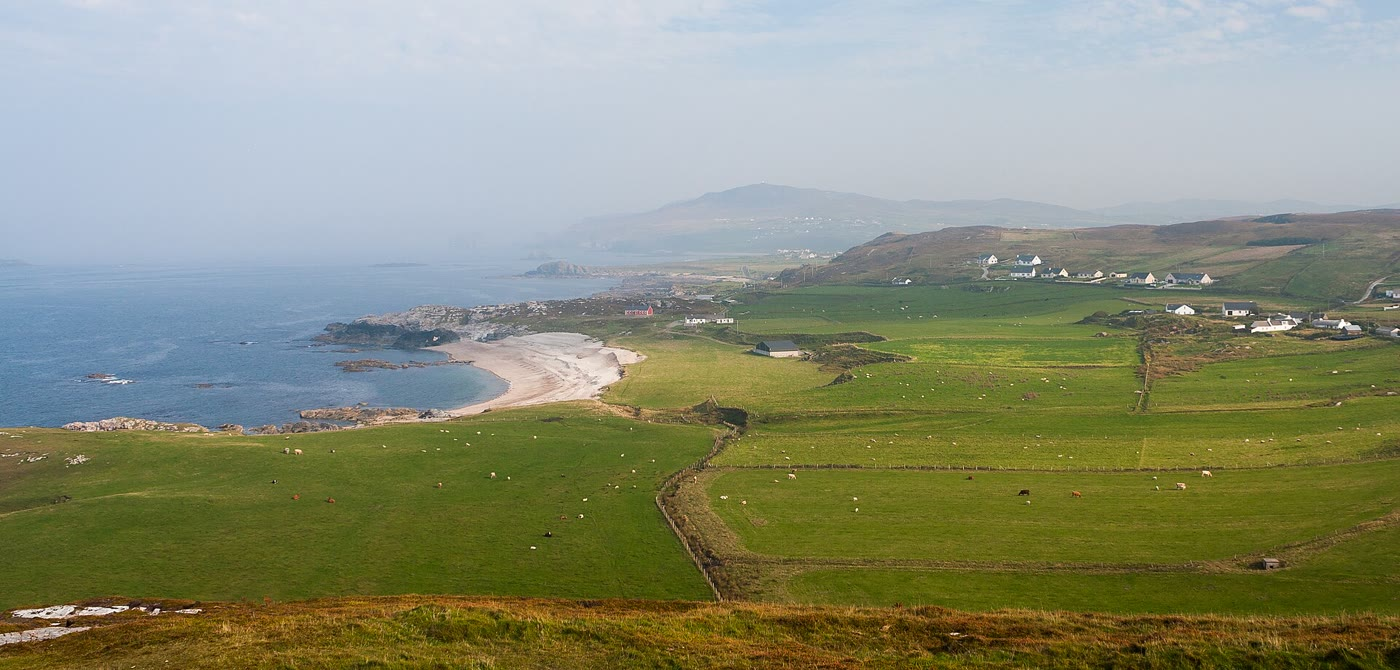
\includegraphics[width=\linewidth]{images/book5/b3-raised-beach-malin.jpg}

{\scriptsize उत्तरी आयरलैंड में, मैलिन हेड के बैलीहिलिन के उठे हुए पुलिन:
पुरानी तटरेखाओं के कंकड़-कटक, जो भूभाग उठने पर समुद्र से ऊपर आ गए
उसकी हिमचादर पिघलने के बाद। फ़ोटो A.~F.~Borchert, CC BY-SA 4.0.}
\end{minipage}
\end{inthefield}
% ledger: photo:b3-raised-beach

\section{पूर्ण-प्रावार संवहन और उसकी गहरी संरचना}

क्या प्रावार एक परत के रूप में संवहन करता है, या दो परतों के रूप में, ऊपर और
नीचे \qty{670}{km} असांतत्य के? टोमोग्राफ़ी (\cref{ch:b3:seismology-imaging} में) आंशिक उत्तर देती है:
कुछ स्लैब असांतत्य के ऊपर समतल हो जाते हैं, अन्य उसे भेदकर निचले प्रावार में धँस जाते हैं,
इसलिए द्रव्यमान उसे पार करता है, और दोनों परतें एक-दूसरे से पूरी तरह बंद नहीं हैं।
गहराई के साथ श्यानता का बढ़ना निचले प्रावार में प्रवाह को धीमा कर देता है,
और स्लैब उसमें प्रवेश करते समय मंद पड़कर मोटे हो जाते हैं।

प्रावार के तल पर टोमोग्राफ़ी दो विस्तृत क्षेत्र दिखाती है, जहाँ S तरंग की गति कम है,
अफ़्रीका के नीचे और प्रशांत महासागर के नीचे, बड़े निम्न-अपरूपण-वेग
प्रांत (LLSVPs)। ये संभवतः रासायनिक रूप से ऊपर के प्रावार से भिन्न हैं
और घने हैं, गर्म प्लूम के बजाय ढेर हैं। पिछले कुछ सौ मिलियन वर्षों के बृहत आग्नेय प्रांत और
किम्बरलाइट मुख्यतः उनकी सीमाओं के ऊपर फूटे,
मानो प्लूम ढेरों के किनारों से उठे हों, जहाँ प्रावार के तल की गर्म
सीमा-परत उनसे टकराकर बहती है।
% ledger: st12:llsvp

\section{अभ्यास}

\begin{exercise}[$\star$]\label{exo:b3:mantle-convection:1}
ऊपरी-प्रावार की \qty{670}{km} मोटी परत की \omterm{def:b3:mantle-convection:rayleigh}{रैले संख्या} परिकलित कीजिए, जिसके लिए
$\rho = \qty{3500}{kg.m^{-3}}$, $g = \qty{9.9}{m.s^{-2}}$, $\alpha =
\qty{3e-5}{K^{-1}}$, $\Delta T = \qty{1000}{K}$, $\kappa =
\qty{e-6}{m^2.s^{-1}}$ और $\eta = \qty{5e20}{Pa.s}$ पर, यह क्रांतिक मान का कितना गुना है,
मुक्त-फिसलन सीमाओं के लिए?
\end{exercise}

\begin{exercise}[$\star$]\label{exo:b3:mantle-convection:2}
प्रावार का \omterm{def:b3:mantle-convection:maxwell}{मैक्सवेल काल} परिकलित कीजिए, जिसकी श्यानता \qty{e21}{Pa.s} और अपरूपण
मापांक \qty{7.7e10}{Pa} है, वर्षों में। क्या प्रावार प्रत्यास्थ रूप से या श्यान रूप से
दिन में दो बार आने वाले पृथ्वी-ज्वार, हिमचादर के पिघलने और
स्लैब के धँसने पर प्रतिक्रिया करता है?
\end{exercise}

\begin{exercise}[$\star$]\label{exo:b3:mantle-convection:3}
$\eta = \qty{e21}{Pa.s}$, $\rho = \qty{3300}{kg.m^{-3}}$ और $g =
\qty{9.8}{m.s^{-2}}$ मानकर, एक समान अर्ध-समष्टि का शिथिलन काल परिकलित कीजिए
तरंगदैर्घ्य 1000 और \qty{3000}{km} वाले भारों के लिए। कौन तेज़ी से पुनर्प्राप्त होता है?
\end{exercise}

\begin{exercise}[$\star$]\label{exo:b3:mantle-convection:4}
$g = \qty{9.8}{m.s^{-2}}$, $\rho_m = \qty{3300}{kg.m^{-3}}$, $\rho_w =
\qty{1030}{kg.m^{-3}}$, $\alpha = \qty{3.1e-5}{K^{-1}}$, $T_m - T_0 =
\qty{1450}{K}$, $\kappa = \qty{0.8e-6}{m^2.s^{-1}}$ और \qty{1}{Myr} $=
\qty{3.156e13}{s}$, \qty{50}{Myr} पर \omterm{prop:b3:mantle-convection:ridge-push}{कटक-धक्का बल} परिकलित कीजिए। यह
\qty{4.6e13}{N.m^{-1}} के स्लैब-खिंचाव से कितने गुना छोटा है?
\end{exercise}

\begin{exercise}[$\star\star$]\label{exo:b3:mantle-convection:5}
प्रावार का एक पिंड, जिसका व्यास \qty{10}{km} है, अपने परिवेश से \qty{300}{K} अधिक गर्म है,
$\rho g\alpha\Delta Td^2/\eta$ की चाल से ऊपर उठता है (मान लीजिए $\rho =
\qty{3300}{kg.m^{-3}}$, $g = \qty{9.8}{m.s^{-2}}$, $\alpha = \qty{3e-5}{K^{-1}}$,
$\eta = \qty{e21}{Pa.s}$, $\kappa = \qty{e-6}{m^2.s^{-1}}$)। (क)~इसका
अपने ही आकार के आर-पार उठने का समय और विसरण काल $d^2/\kappa$ परिकलित कीजिए, और
दिखाइए कि उनका अनुपात उसकी \omterm{def:b3:mantle-convection:rayleigh}{रैले संख्या} है। (ख)~क्या यह पहले उठता है या ठंडा होता है? (ग)~
उसकी \omterm{def:b3:mantle-convection:rayleigh}{रैले संख्या} 657.5 तक पहुँचने के लिए यह कितना बड़ा होना चाहिए?
\end{exercise}

\begin{exercise}[$\star\star$]\label{exo:b3:mantle-convection:6}
\qty{2891}{km} गहरी परत के लिए, जहाँ $\mathrm{Ra} = \num{e7}$ है और $\kappa =
\qty{e-6}{m^2.s^{-1}}$, $k = \qty{3.1}{W.m^{-1}.K^{-1}}$, $\Delta T =
\qty{1450}{K}$ और $\mathrm{Ra}_c = 657.5$, सीमा-परत की
मोटाई, \omterm{def:b3:mantle-convection:nusselt}{नुसेल्ट संख्या}, \unit{cm/yr} में वेग-स्केल और ऊष्मा-प्रवाह
परिकलित कीजिए।
\end{exercise}

\begin{exercise}[$\star\star$]\label{exo:b3:mantle-convection:7}
एक काल्पनिक हॉटस्पॉट-उभार का, पथ के आर-पार, अनुप्रस्थ-काट
क्षेत्रफल \qty{8e8}{m^2} है, और उसके ऊपर की प्लेट \qty{9}{cm/yr} से चलती है। मान लीजिए $\rho_m - \rho_w =
\qty{2270}{kg.m^{-3}}$ लेकर इसका उत्प्लावन अभिवाह, और $c_p =
\qty{1170}{J.kg^{-1}.K^{-1}}$ और $\alpha = \qty{3.1e-5}{K^{-1}}$ के साथ इसका ऊष्मा-प्रवाह परिकलित कीजिए।
यह पृथ्वी के \qty{46.7}{TW} का कितना अंश है?
\end{exercise}

\begin{exercise}[$\star\star$]\label{exo:b3:mantle-convection:8}
त्रिज्या \qty{400}{km} वाला एक प्लूम-शीर्ष, जो प्रावार से
\qty{30}{kg.m^{-3}} हल्का है, श्यानता \qty{e21}{Pa.s} वाले प्रावार से होकर ऊपर उठता है।
स्टोक्स के नियम से \unit{m/yr} में इसकी चाल, और वह समय जिसमें यह
\qty{2000}{km} ऊपर उठता है, परिकलित कीजिए।
\end{exercise}

\begin{exercise}[$\star\star$]\label{exo:b3:mantle-convection:9}
एक क्षेत्र, जब उसकी हिमचादर पिघली, \qty{10}{kyr} पहले, \qty{300}{m} दब गया था,
और $\tau = \qty{4.4}{kyr}$ के साथ शिथिल होता है। आज बचा अवधसान और
वर्तमान उत्थान-दर परिकलित कीजिए। उमेओ के निकट मापे गए
\qty{10.3}{mm/yr} से तुलना कीजिए।
\end{exercise}

\begin{exercise}[$\star\star\star$]\label{exo:b3:mantle-convection:10}
(क)~$F_{rp}$ का व्यंजक, जो
\cref{prop:b3:mantle-convection:ridge-push} की उपपत्ति में है, दिखाइए कि पहला पद,
$\tfrac12(\rho_m - \rho_w)gw^2$, कोष्ठक का दूसरा पद है। (ख)~दिखाइए कि
$\int_0^\infty x\operatorname{erfc}x\,\mathrm dx = 1/4$ है, भागों द्वारा समाकलन करके।
(ग)~अभ्यास 4 के मानों से \qty{100}{Myr} पर दोनों पद परिकलित कीजिए।
\end{exercise}

\begin{exercise}[$\star\star\star$]\label{exo:b3:mantle-convection:11}
दिखाइए कि $f(k) = (\pi^2 + k^2)^3/k^2$ न्यूनतम होता है, $k = \pi/\sqrt2$ पर, जहाँ
उसका मान $27\pi^4/4$ होता है। आरंभ पर संवहन-कोष्ठों की एक जोड़ी की
चौड़ाई $d$ की इकाइयों में और एक कोष्ठ की चौड़ाई निकालिए।
\end{exercise}

\begin{exercise}[$\star\star\star$]\label{exo:b3:mantle-convection:12}
लंबाई \qty{6000}{km} वाली एक प्लेट प्रावार की एक परत पर \qty{6}{cm/yr} से चलती है,
जो \qty{150}{km} मोटी और श्यानता \qty{e20}{Pa.s} वाली है, और जिसका तल स्थिर है। (क)~
\omterm{def:b3:mantle-convection:basal-drag}{आधारी कर्षण} \unit{MPa} में और प्लेट की प्रति इकाई लंबाई पर कर्षण बल परिकलित कीजिए।
(ख)~\qty{3.8e12}{N.m^{-1}} के \omterm{prop:b3:mantle-convection:ridge-push}{कटक-धक्का बल} और
\qty{4.6e13}{N.m^{-1}} के स्लैब-खिंचाव से तुलना कीजिए। (ग)~यदि स्लैब-खिंचाव का दसवाँ भाग प्लेट तक पहुँचे,
किस चाल पर कर्षण चालक बलों को संतुलित करता है?
\end{exercise}

\section{समस्या: झील आर्डो का प्रतिक्षेप}

\begin{problem}[{सप्ताहांत समस्या --- एक काल्पनिक झील-द्रोणी का प्रतिक्षेप,
उसके नीचे के प्रावार की श्यानता, और वह संवहन
जिसे यह श्यानता संभव बनाती है}]
\label{pb:b3:mantle-convection:1}
% values: calc/ch06.py; gia_relaxation.py, convection_scaling.py
झील आर्डो, एक काल्पनिक झील, \qty{250}{km} चौड़ी एक द्रोणी को भरती थी, जिसे
एक हिमचादर ने बाँध रखा था, और वह लगभग पचास हज़ार वर्ष तक \qty{300}{m} गहरी रही। चौदह
हज़ार वर्ष पहले हिम-बाँध टूटा और झील कुछ सप्ताहों में निकल गई। उसकी
सबसे ऊँची तटरेखा, जो बनने के समय समतल थी, अब झुकी है; द्रोणी में बची छोटी झीलों की
काल-निर्धारित तटरेखाएँ बताती हैं कि निकासी के बाद से केंद्र का उत्थान
कगार के सापेक्ष कितना हुआ है, जो लगभग नहीं हिला:

\smallskip
\begin{center}\small
\begin{tabular}{lcccccc}
\hline
निकासी के बाद का समय (kyr) & 1 & 2 & 4 & 6 & 9 & 14\\
केंद्र का उत्थान (m) & 11.5 & 21.6 & 38.0 & 50.5 & 64.0 & 77.2\\
\hline
\end{tabular}
\end{center}
\smallskip

मान लीजिए $\rho_w = \qty{1000}{kg.m^{-3}}$, $\rho_m = \qty{3300}{kg.m^{-3}}$, $g =
\qty{9.8}{m.s^{-2}}$, \qty{1}{yr} $= \qty{3.156e7}{s}$, और प्रावार को
एक समान श्यान अर्ध-समष्टि मानिए।

\medskip\noindent\textbf{भाग I --- भार।}
\begin{enumerate}
  \item झील द्वारा उसके तल पर लगाया दाब परिकलित कीजिए।
  \item समस्थितिक साम्य पर तल का अवनमन परिकलित कीजिए, और बताइए
        कि उसमें भूपर्पटी का नहीं, प्रावार का घनत्व क्यों आता है।
  \item झील को एक चकती मानकर उसके जल का द्रव्यमान परिकलित कीजिए।
  \item समझाइए कि सबसे ऊँची तटरेखा अब क्यों झुकी है, और उसकी माध्य
        ढाल कगार से केंद्र तक, मीटर प्रति किलोमीटर में, परिकलित कीजिए।
  \item अवनमन को एक हार्मोनिक मानिए जिसका अवनमित अर्ध-भाग
        $-\lambda/4$ से $\lambda/4$ तक झील को घेरता है। $\lambda$ और $k =
        2\pi/\lambda$ दीजिए।
  \item ऐसे भार के नीचे का प्रवाह किस गहराई पर गुणक
        $e$ से क्षय होता है?
\end{enumerate}

\medskip\noindent\textbf{भाग II --- शिथिलन काल।}
\begin{enumerate}[resume]
  \item मान लीजिए कि झील साम्य तक पहुँच चुकी थी, तो
        सारणी की प्रत्येक तिथि पर बचा अवनमन परिकलित कीजिए।
  \item सिद्ध कीजिए कि यदि अवनमन घातांकीय रूप से क्षय होता है, तो उसका लघुगणक
        समय के साथ रैखिक रूप से घटता है।
  \item तिथियों 1 और \qty{14}{kyr} से $\tau$ परिकलित कीजिए।
  \item उस $\tau$ से \qty{6}{kyr} पर उत्थान का पूर्वानुमान लगाइए और
        सारणी से तुलना कीजिए।
  \item आज बचा अवनमन और केंद्र की वर्तमान उत्थान-दर
        \unit{mm/yr} में परिकलित कीजिए।
  \item अभी कितना उत्थान शेष है?
  \item कितने और वर्षों में उत्थान-दर घटकर
        \qty{0.5}{mm/yr} से नीचे आ जाएगी?
\end{enumerate}

\medskip\noindent\textbf{भाग III --- श्यानता।}
\begin{enumerate}[resume]
  \item $\tau$ से अर्ध-समष्टि की श्यानता परिकलित कीजिए।
  \item इसकी तुलना फ़ेनोस्कैंडिया के नीचे पाई गई ऊपरी-प्रावार श्यानताओं से कीजिए, जो
        \num{3.4e20} से \qty{1e21}{Pa.s} के बीच हैं। प्रावार का कौन-सा भाग
        झील आर्डो का प्रतिक्षेप नमूना लेता है?
  \item उस श्यानता के साथ, तरंगदैर्घ्य में \qty{3000}{km} वाले भार का
        शिथिलन काल परिकलित कीजिए। उस आकार की वास्तविक हिमचादर इससे
        अधिक धीरे क्यों शिथिल होगी?
  \item प्रत्यास्थ स्थलमंडल, जिसे यहाँ अनदेखा किया गया है, केवल
        \qty{250}{km} चौड़े भार के प्रतिक्षेप पर क्या प्रभाव डालता है?
  \item $\mu = \qty{7.7e10}{Pa}$ के साथ प्रावार का \omterm{def:b3:mantle-convection:maxwell}{मैक्सवेल काल} परिकलित कीजिए,
        और बताइए कि श्यान मॉडल उचित था या नहीं।
  \item प्रश्न 7 की मान्यता की जाँच कीजिए: झील के खड़े रहने के दौरान साम्य
        अवनमन का कौन-सा भाग प्राप्त हुआ?
  \item $\log_{10}\eta$ कितना बदलेगा यदि $\lambda$ को
        \qty{250}{km} लिया जाए?
\end{enumerate}

\medskip\noindent\textbf{भाग IV --- संवहन।} ऊपरी-प्रावार की एक परत लीजिए
\qty{670}{km} गहरी, जिसका $\rho = \qty{3700}{kg.m^{-3}}$ और $g =
\qty{9.9}{m.s^{-2}}$, $\alpha = \qty{3.1e-5}{K^{-1}}$, $\Delta T =
\qty{1450}{K}$, $\kappa = \qty{e-6}{m^2.s^{-1}}$, $k = \qty{3.1}{W.m^{-1}.K^{-1}}$
और भाग III वाली श्यानता।
\begin{enumerate}[resume]
  \item परत की \omterm{def:b3:mantle-convection:rayleigh}{रैले संख्या} परिकलित कीजिए।
  \item यह क्रांतिक मान से कितने गुना है ($\mathrm{Ra}_c = 657.5$)?
  \item सीमा-परत की मोटाई और \omterm{def:b3:mantle-convection:nusselt}{नुसेल्ट संख्या} परिकलित कीजिए।
  \item \unit{cm/yr} में वेग-स्केल परिकलित कीजिए, और
        प्लेट की 1 से \qty{7.5}{cm/yr} तक की चालों से तुलना कीजिए।
  \item ऊष्मा-प्रवाह परिकलित कीजिए, और दो कारण दीजिए कि वह पृथ्वी के
        माध्य, \qty{92}{mW.m^{-2}}, से क्यों कम है।
  \item झील आर्डो के नीचे ऊपरी-प्रावार की श्यानता का $\log_{10}$
        $\eta$ का \unit{Pa.s} में मान दीजिए।
\end{enumerate}
\end{problem}
